% !TEX root=../report.tex

\section{Experiments}
\label{sec:experiment}


\subsection{One Agent vs. One Adversary Results}
\label{sec:experiment:1vs1}


\begin{figure}[h]
  \centering

  \begin{subfigure}[h]{\figscale\linewidth}
    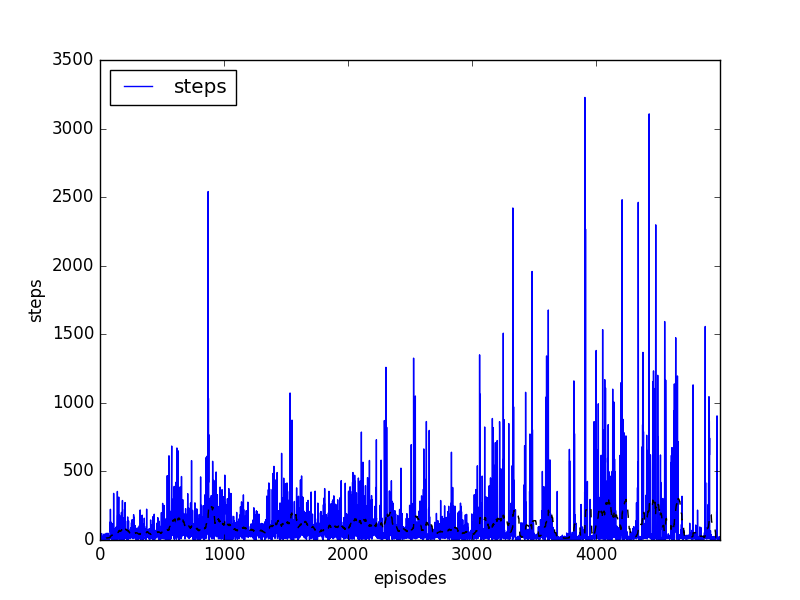
\includegraphics[trim=10 10 10 10,clip,width=\linewidth]
    {../results/dqn_1vs1/steps.png}
    \caption{Number of steps per episode over training episode for DQN.}
    \label{fig:dqn-1vs1-steps}
  \end{subfigure}
  ~
  \begin{subfigure}[h]{\figscale\linewidth}
    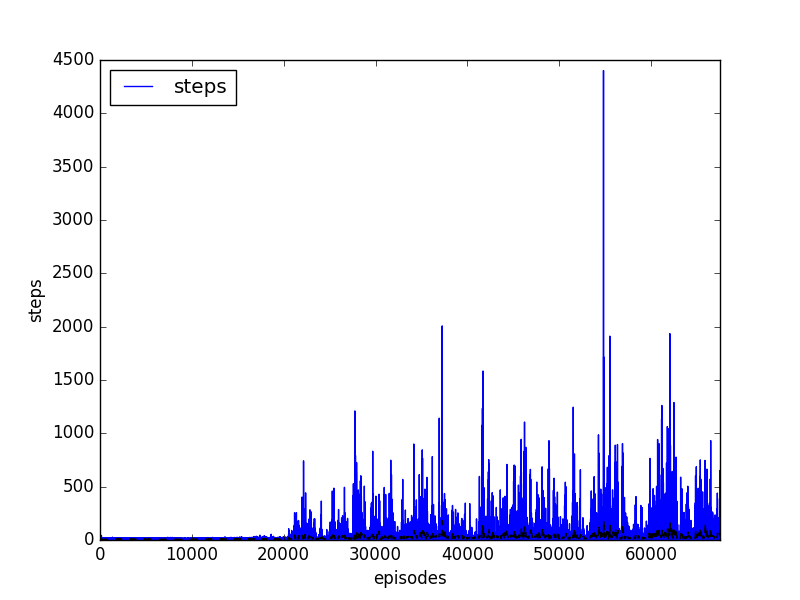
\includegraphics[trim=10 10 10 10,clip,width=\linewidth]
    {../results/ddpg_1vs1/steps.png}
    \caption{Number of steps per episode over training episode for DDPG.}
    \label{fig:ddpg-1vs1-steps}
  \end{subfigure}
  ~
  \begin{subfigure}[h]{\figscale\linewidth}
    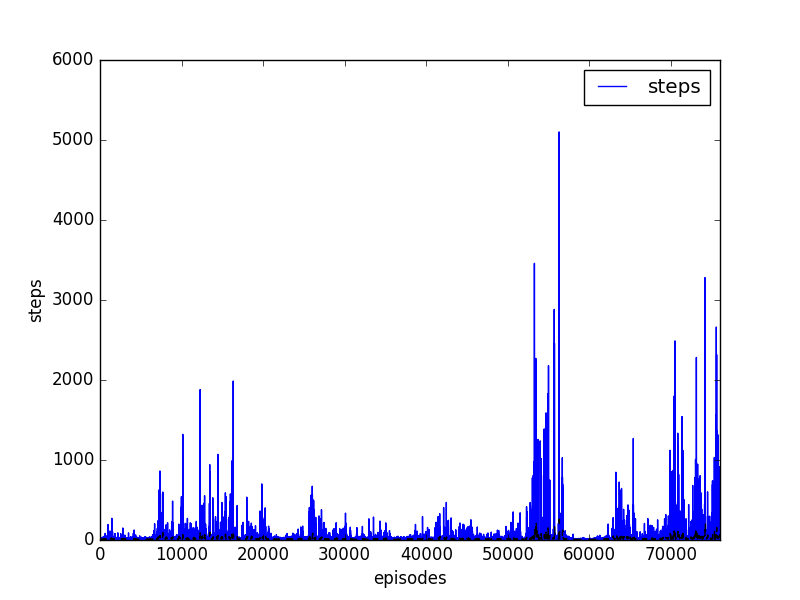
\includegraphics[trim=10 10 10 10,clip,width=\linewidth]
    {../results/maddpg_1vs1/steps.png}
    \caption{Number of steps per episode over training episode for MADDPG.}
    \label{fig:maddpg-1vs1-steps}
  \end{subfigure}

  \begin{subfigure}[h]{\figscale\linewidth}
    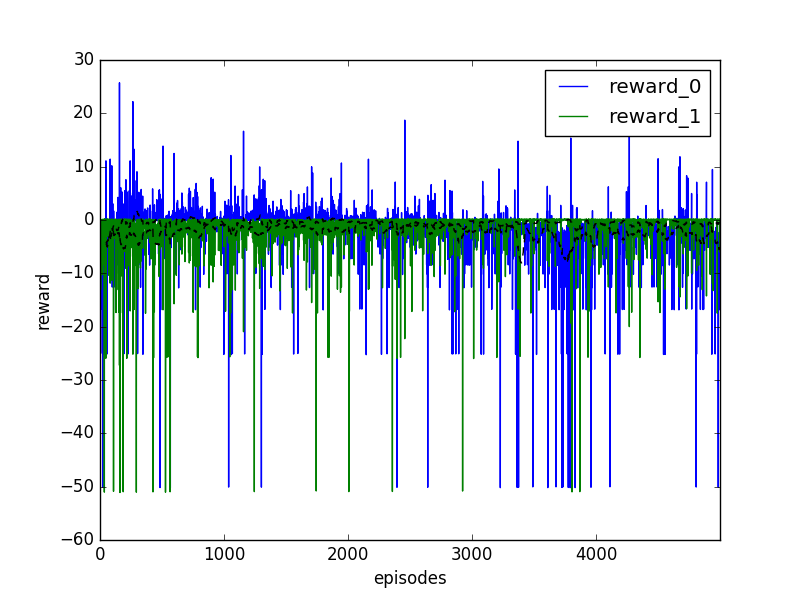
\includegraphics[trim=10 10 10 10,clip,width=\linewidth]
    {../results/dqn_1vs1/reward.png}
    \caption{Cumulative reward per episode over training episode for DQN.}
    \label{fig:dqn-1vs1-reward}
  \end{subfigure}
  ~
  \begin{subfigure}[h]{\figscale\linewidth}
    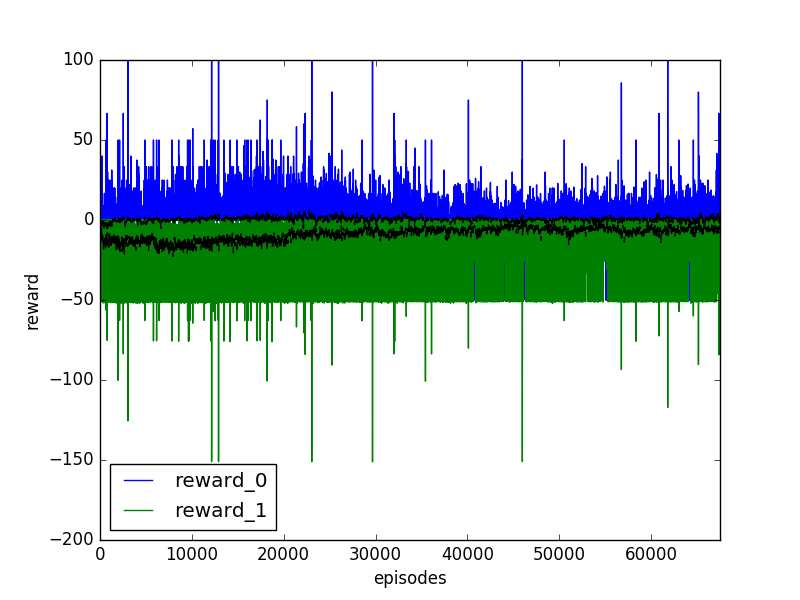
\includegraphics[trim=10 10 10 10,clip,width=\linewidth]
    {../results/ddpg_1vs1/reward.png}
    \caption{Cumulative reward per episode over training episode for DDPG.}
    \label{fig:ddpg-1vs1-reward}
  \end{subfigure}
  ~
  \begin{subfigure}[h]{\figscale\linewidth}
    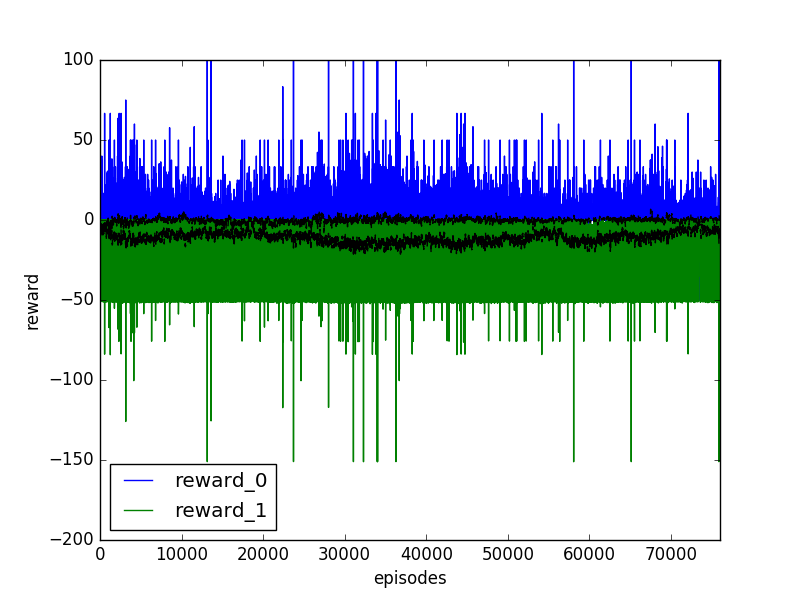
\includegraphics[trim=10 10 10 10,clip,width=\linewidth]
    {../results/maddpg_1vs1/reward.png}
    \caption{Cumulative reward per episode over training episode for MADDPG.}
    \label{fig:maddpg-1vs1-reward}
  \end{subfigure}

  \begin{subfigure}[h]{\figscale\linewidth}
    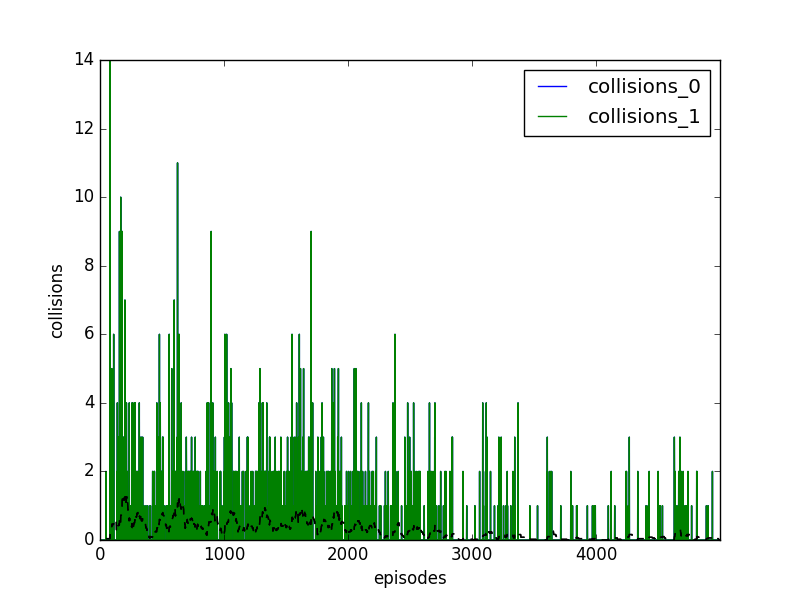
\includegraphics[trim=10 10 10 10,clip,width=\linewidth]
    {../results/dqn_1vs1/collisions.png}
    \caption{Number of collisions per episode over training episode for DQN.}
    \label{fig:dqn-1vs1-collisions}
  \end{subfigure}
  ~
  \begin{subfigure}[h]{\figscale\linewidth}
    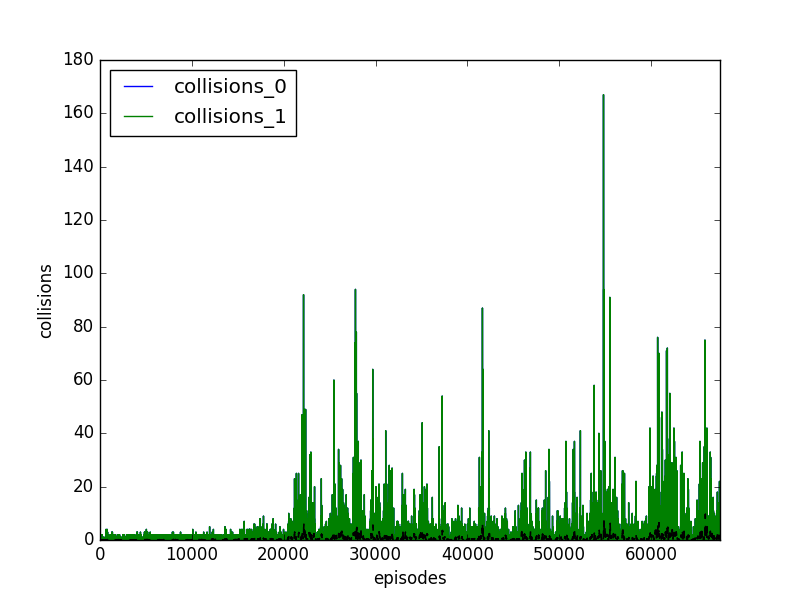
\includegraphics[trim=10 10 10 10,clip,width=\linewidth]
    {../results/ddpg_1vs1/collisions.png}
    \caption{Number of collisions per episode over training episode for DDPG.}
    \label{fig:ddpg-1vs1-collisions}
  \end{subfigure}
  ~
  \begin{subfigure}[h]{\figscale\linewidth}
    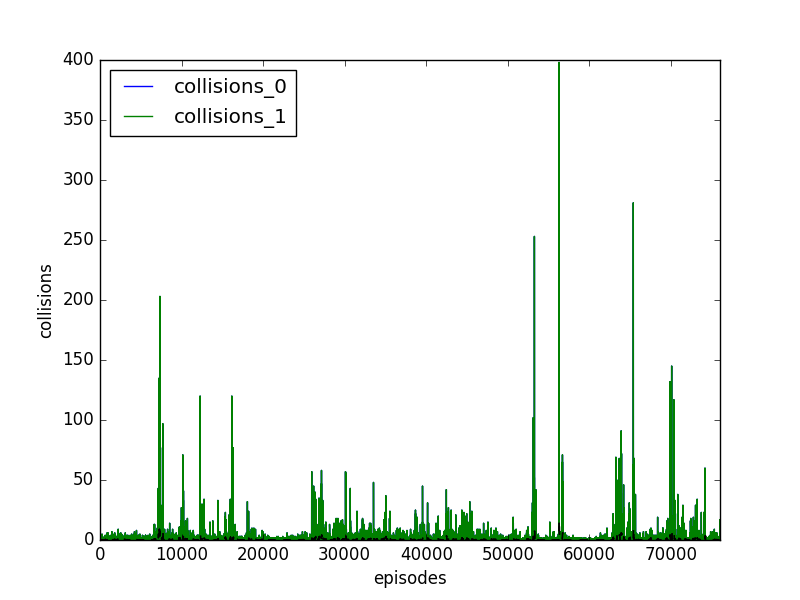
\includegraphics[trim=10 10 10 10,clip,width=\linewidth]
    {../results/maddpg_1vs1/collisions.png}
    \caption{Number of collisions per episode over training episode for MADDPG.}
    \label{fig:maddpg-1vs1-collisions}
  \end{subfigure}

  \begin{subfigure}[h]{\figscale\linewidth}
    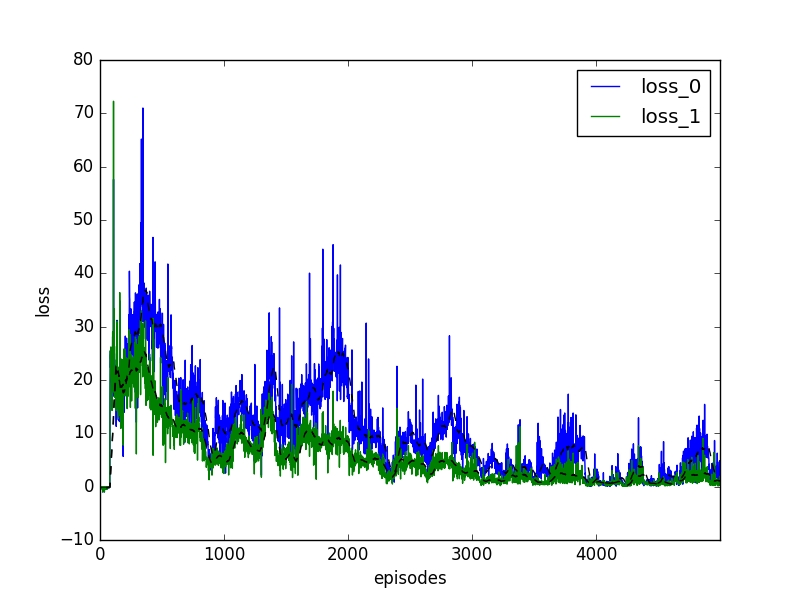
\includegraphics[trim=10 10 10 10,clip,width=\linewidth]
    {../results/dqn_1vs1/loss.png}
    \caption{Average loss per episode over training episode for DQN.}
    \label{fig:dqn-1vs1-loss}
  \end{subfigure}
  ~
  \begin{subfigure}[h]{\figscale\linewidth}
    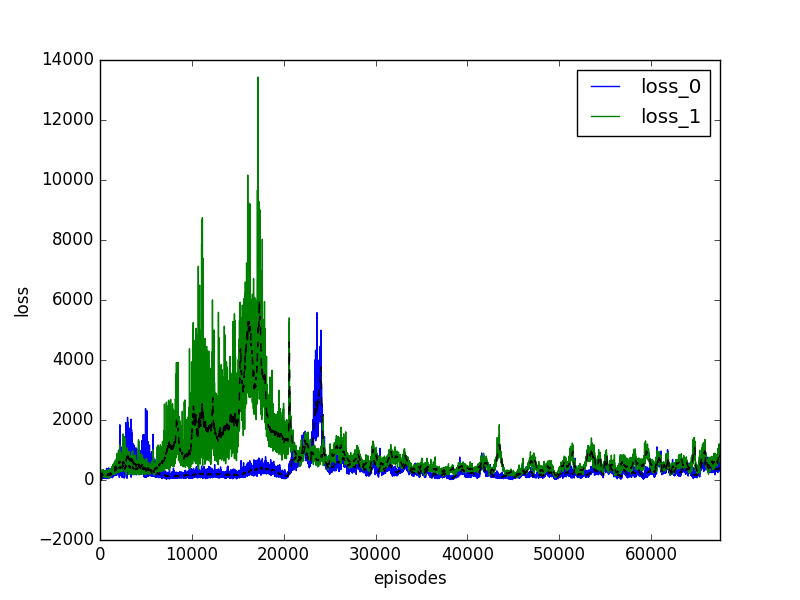
\includegraphics[trim=10 10 10 10,clip,width=\linewidth]
    {../results/ddpg_1vs1/loss.png}
    \caption{Average loss per episode over training episode for DDPG.}
    \label{fig:ddpg-1vs1-loss}
  \end{subfigure}
  ~
  \begin{subfigure}[h]{\figscale\linewidth}
    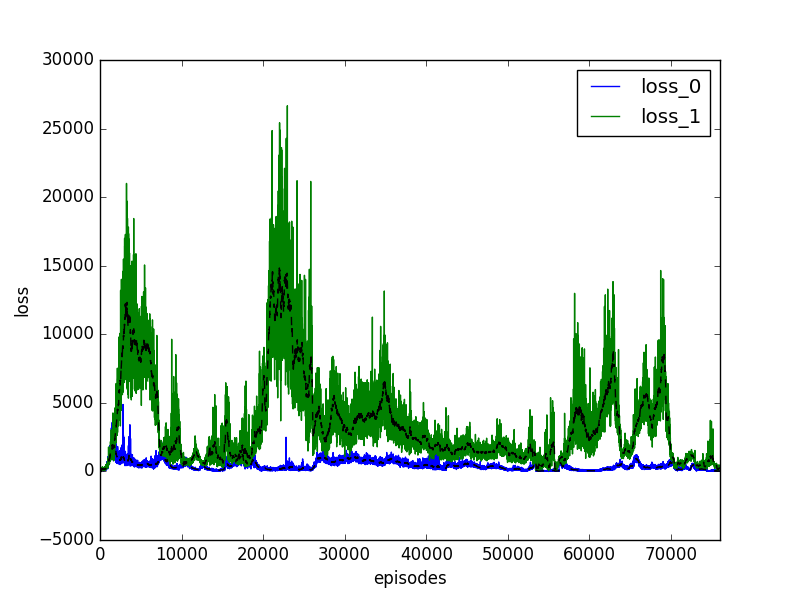
\includegraphics[trim=10 10 10 10,clip,width=\linewidth]
    {../results/maddpg_1vs1/loss.png}
    \caption{Average loss per episode over training episode for MADDPG.}
    \label{fig:maddpg-1vs1-loss}
  \end{subfigure}


  \caption{Results for predator-pray with one agent vs. one adversary}
  \label{fig:1vs1}
\end{figure}
\FloatBarrier


\subsection{Two Agents vs. One Adversary Results}
\label{sec:experiment:1vs2}


\begin{figure}[h]
  \centering

  \begin{subfigure}[h]{\figscale\linewidth}
    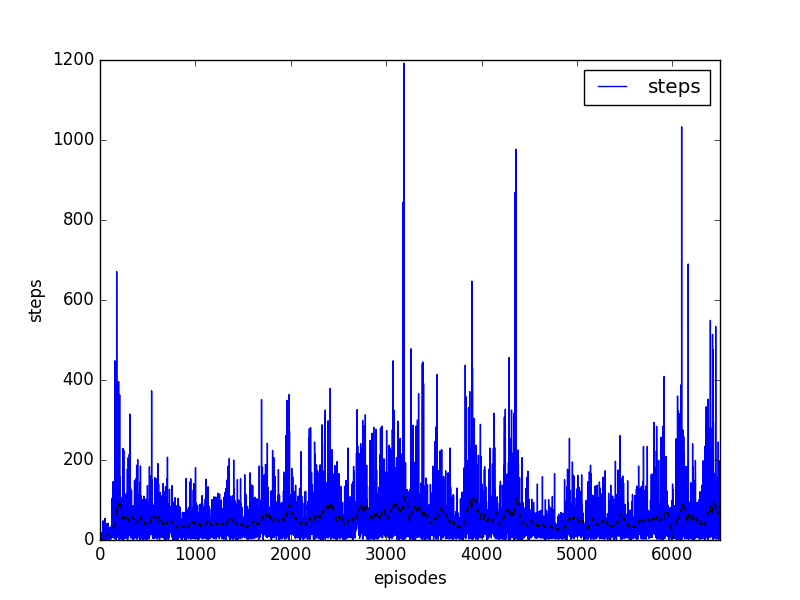
\includegraphics[trim=10 10 10 10,clip,width=\linewidth]
    {../results/dqn_1vs2/steps.png}
    \caption{Number of steps per episode over training episode for DQN.}
    \label{fig:dqn-1vs2-steps}
  \end{subfigure}
  ~
  \begin{subfigure}[h]{\figscale\linewidth}
    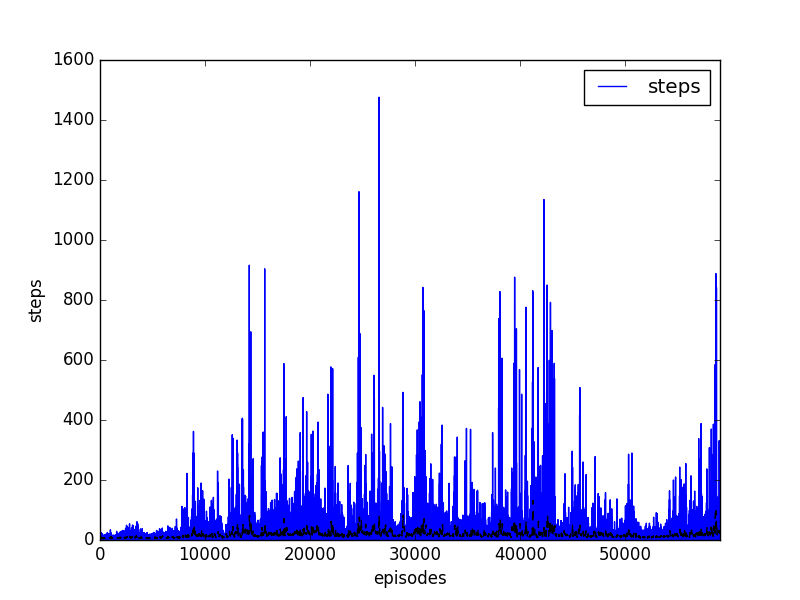
\includegraphics[trim=10 10 10 10,clip,width=\linewidth]
    {../results/ddpg_1vs2/steps.png}
    \caption{Number of steps per episode over training episode for DDPG.}
    \label{fig:ddpg-1vs2-steps}
  \end{subfigure}
  ~
  \begin{subfigure}[h]{\figscale\linewidth}
    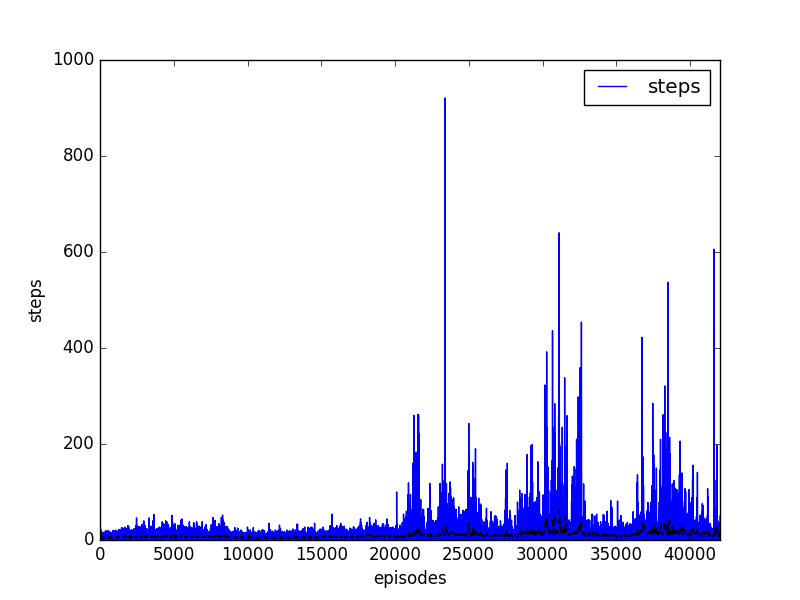
\includegraphics[trim=10 10 10 10,clip,width=\linewidth]
    {../results/maddpg_1vs2/steps.png}
    \caption{Number of steps per episode over training episode for MADDPG.}
    \label{fig:maddpg-1vs2-steps}
  \end{subfigure}

  \begin{subfigure}[h]{\figscale\linewidth}
    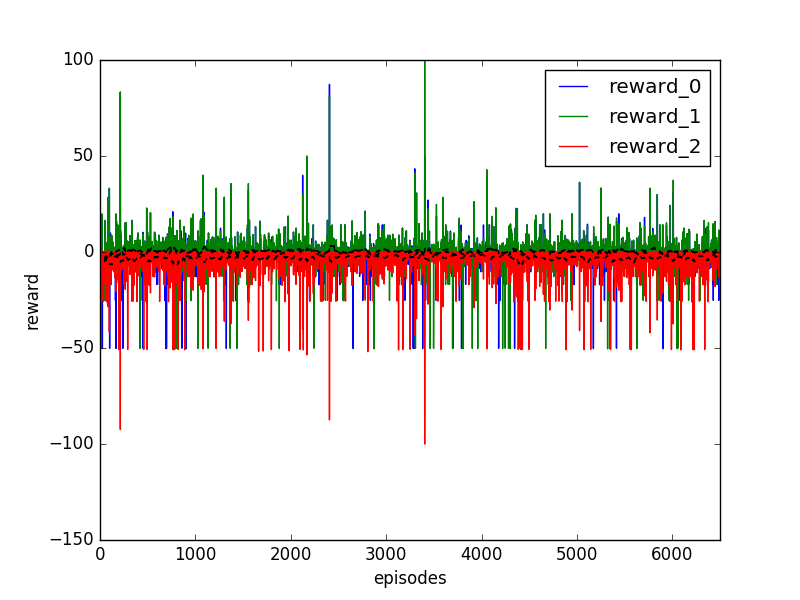
\includegraphics[trim=10 10 10 10,clip,width=\linewidth]
    {../results/dqn_1vs2/reward.png}
    \caption{Cumulative reward per episode over training episode for DQN.}
    \label{fig:dqn-1vs2-reward}
  \end{subfigure}
  ~
  \begin{subfigure}[h]{\figscale\linewidth}
    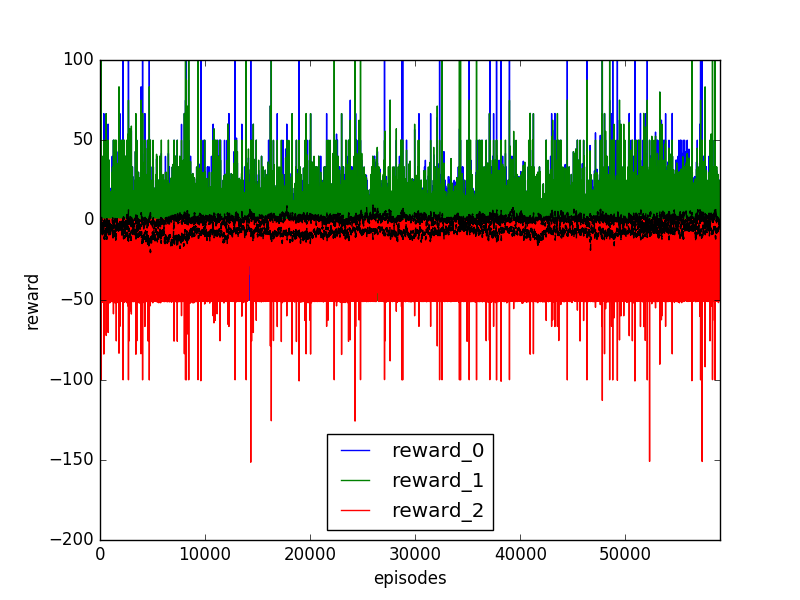
\includegraphics[trim=10 10 10 10,clip,width=\linewidth]
    {../results/ddpg_1vs2/reward.png}
    \caption{Cumulative reward per episode over training episode for DDPG.}
    \label{fig:ddpg-1vs2-reward}
  \end{subfigure}
  ~
  \begin{subfigure}[h]{\figscale\linewidth}
    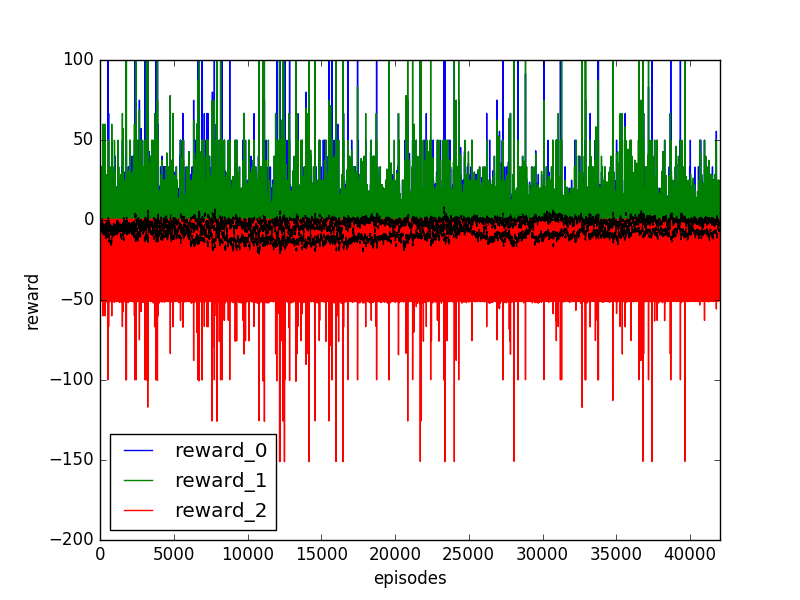
\includegraphics[trim=10 10 10 10,clip,width=\linewidth]
    {../results/maddpg_1vs2/reward.png}
    \caption{Cumulative reward per episode over training episode for MADDPG.}
    \label{fig:maddpg-1vs2-reward}
  \end{subfigure}

  \begin{subfigure}[h]{\figscale\linewidth}
    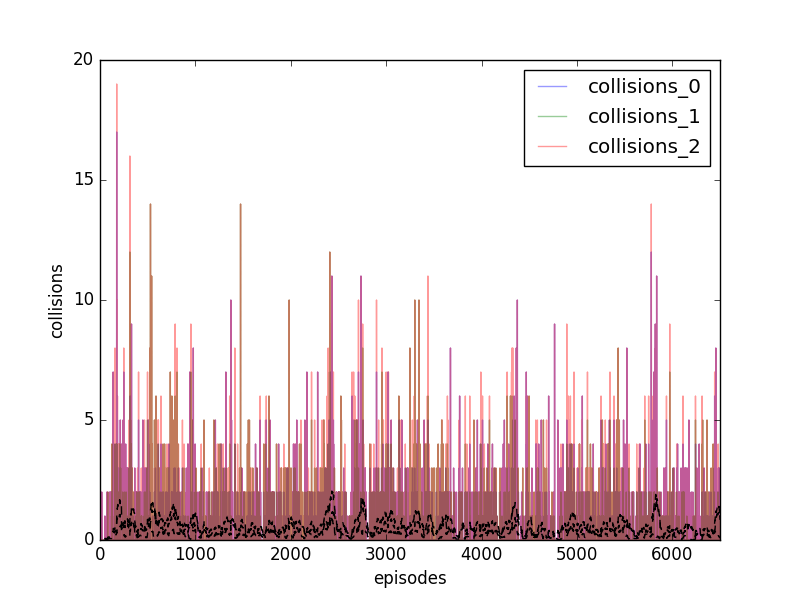
\includegraphics[trim=10 10 10 10,clip,width=\linewidth]
    {../results/dqn_1vs2/collisions.png}
    \caption{Number of collisions per episode over training episode for DQN.}
    \label{fig:dqn-1vs2-collisions}
  \end{subfigure}
  ~
  \begin{subfigure}[h]{\figscale\linewidth}
    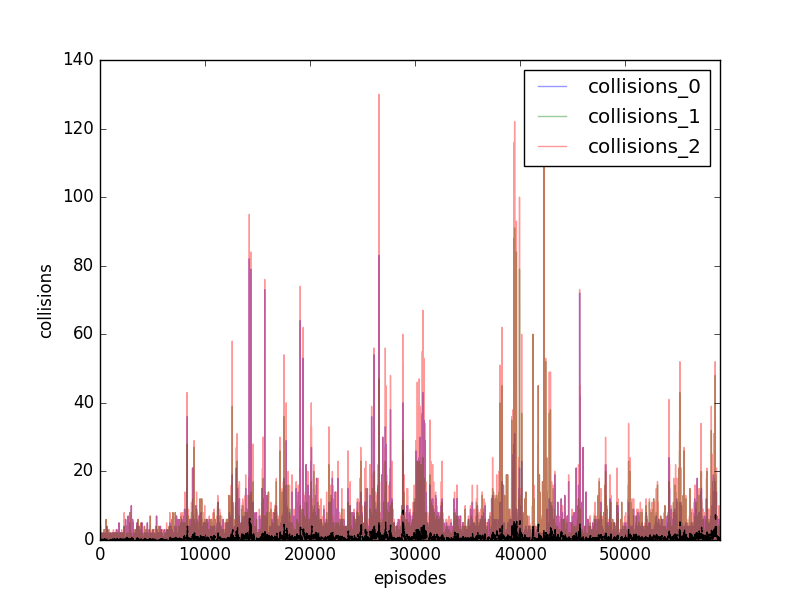
\includegraphics[trim=10 10 10 10,clip,width=\linewidth]
    {../results/ddpg_1vs2/collisions.png}
    \caption{Number of collisions per episode over training episode for DDPG.}
    \label{fig:ddpg-1vs2-collisions}
  \end{subfigure}
  ~
  \begin{subfigure}[h]{\figscale\linewidth}
    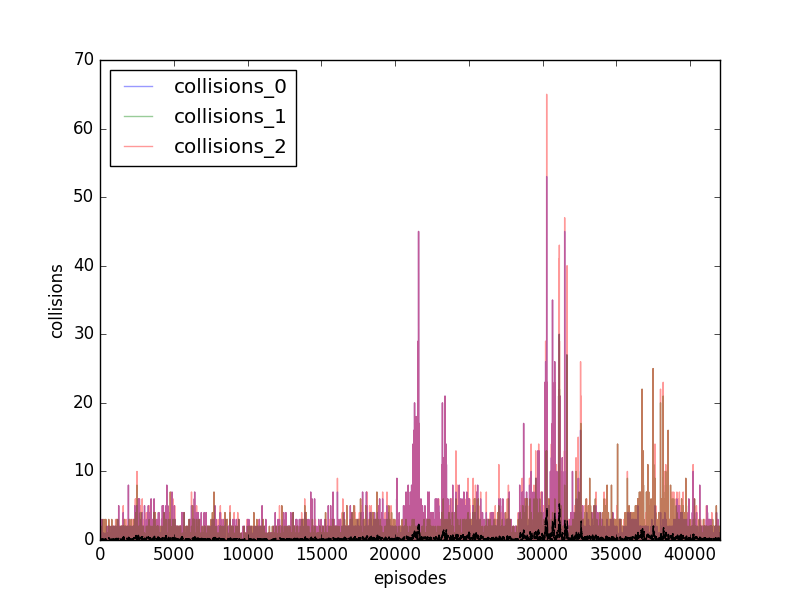
\includegraphics[trim=10 10 10 10,clip,width=\linewidth]
    {../results/maddpg_1vs2/collisions.png}
    \caption{Number of collisions per episode over training episode for MADDPG.}
    \label{fig:maddpg-1vs2-collisions}
  \end{subfigure}

  \begin{subfigure}[h]{\figscale\linewidth}
    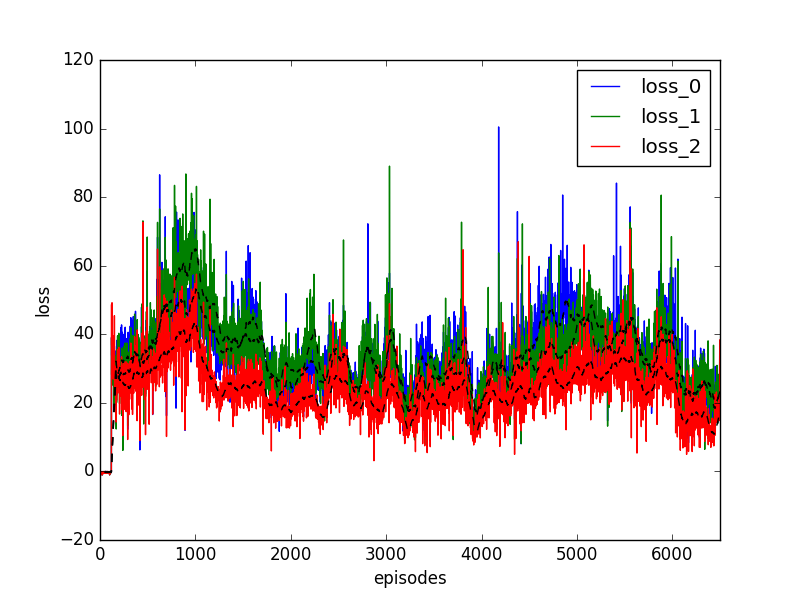
\includegraphics[trim=10 10 10 10,clip,width=\linewidth]
    {../results/dqn_1vs2/loss.png}
    \caption{Average loss per episode over training episode for DQN.}
    \label{fig:dqn-1vs2-loss}
  \end{subfigure}
  ~
  \begin{subfigure}[h]{\figscale\linewidth}
    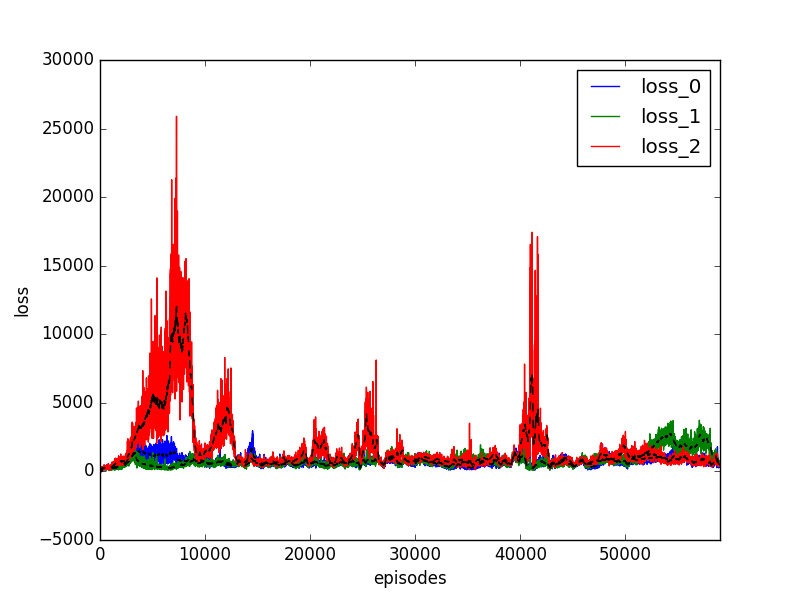
\includegraphics[trim=10 10 10 10,clip,width=\linewidth]
    {../results/ddpg_1vs2/loss.png}
    \caption{Average loss per episode over training episode for DDPG.}
    \label{fig:ddpg-1vs2-loss}
  \end{subfigure}
  ~
  \begin{subfigure}[h]{\figscale\linewidth}
    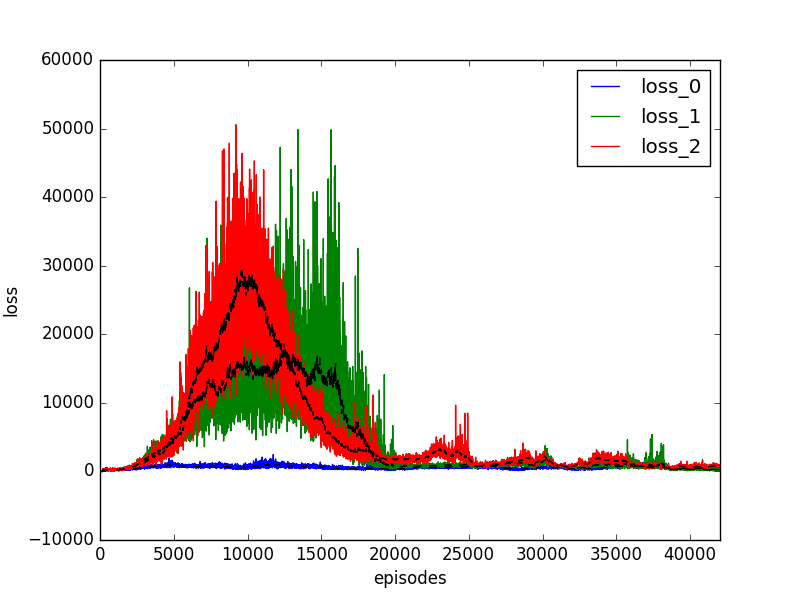
\includegraphics[trim=10 10 10 10,clip,width=\linewidth]
    {../results/maddpg_1vs2/loss.png}
    \caption{Average loss per episode over training episode for MADDPG.}
    \label{fig:maddpg-1vs2-loss}
  \end{subfigure}


  \caption{Results for predator-pray with two agents vs. one adversary}
  \label{fig:1vs2}
\end{figure}
\FloatBarrier


\subsection{One Agent vs. Two Adversaries Results}
\label{sec:experiment:2vs1}


\begin{figure}[h]
  \centering

  \begin{subfigure}[h]{\figscale\linewidth}
    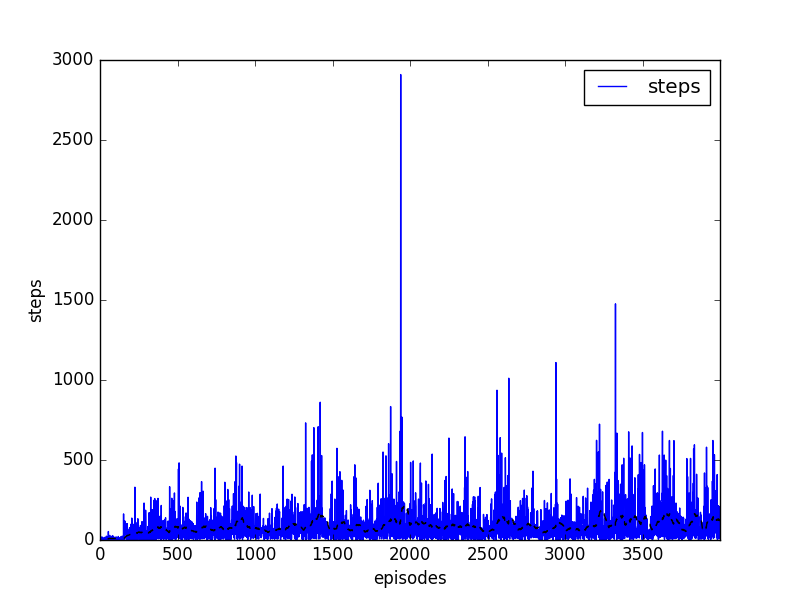
\includegraphics[trim=10 10 10 10,clip,width=\linewidth]
    {../results/dqn_2vs1/steps.png}
    \caption{Number of steps per episode over training episode for DQN.}
    \label{fig:dqn-2vs1-steps}
  \end{subfigure}
  ~
  \begin{subfigure}[h]{\figscale\linewidth}
    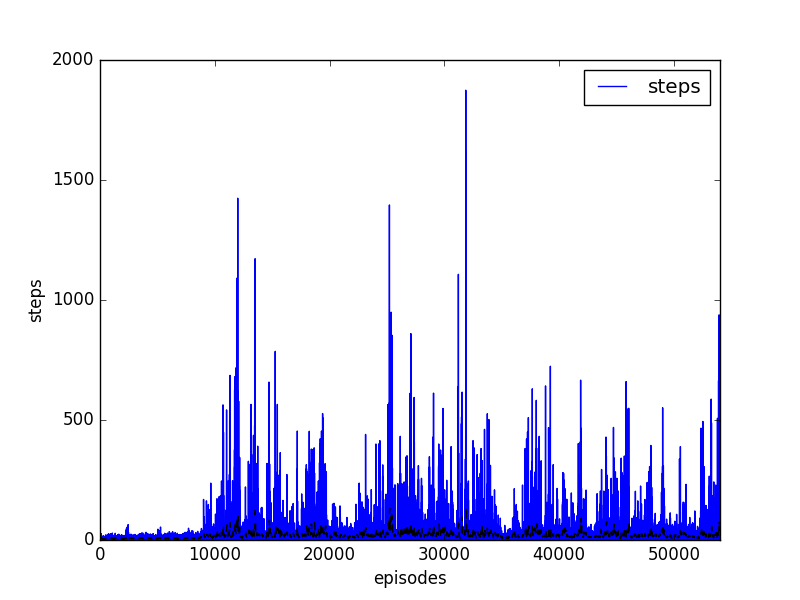
\includegraphics[trim=10 10 10 10,clip,width=\linewidth]
    {../results/ddpg_2vs1/steps.png}
    \caption{Number of steps per episode over training episode for DDPG.}
    \label{fig:ddpg-2vs1-steps}
  \end{subfigure}
  ~
  \begin{subfigure}[h]{\figscale\linewidth}
    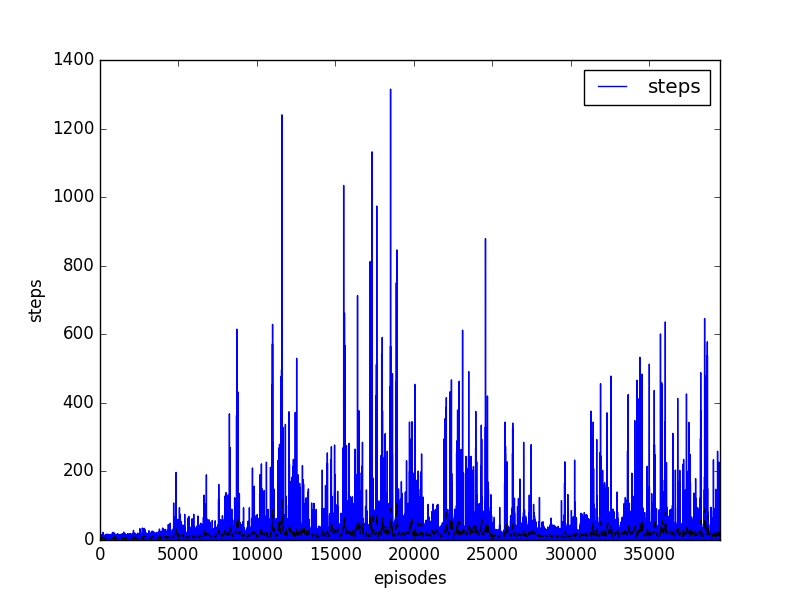
\includegraphics[trim=10 10 10 10,clip,width=\linewidth]
    {../results/maddpg_2vs1/steps.png}
    \caption{Number of steps per episode over training episode for MADDPG.}
    \label{fig:maddpg-2vs1-steps}
  \end{subfigure}

  \begin{subfigure}[h]{\figscale\linewidth}
    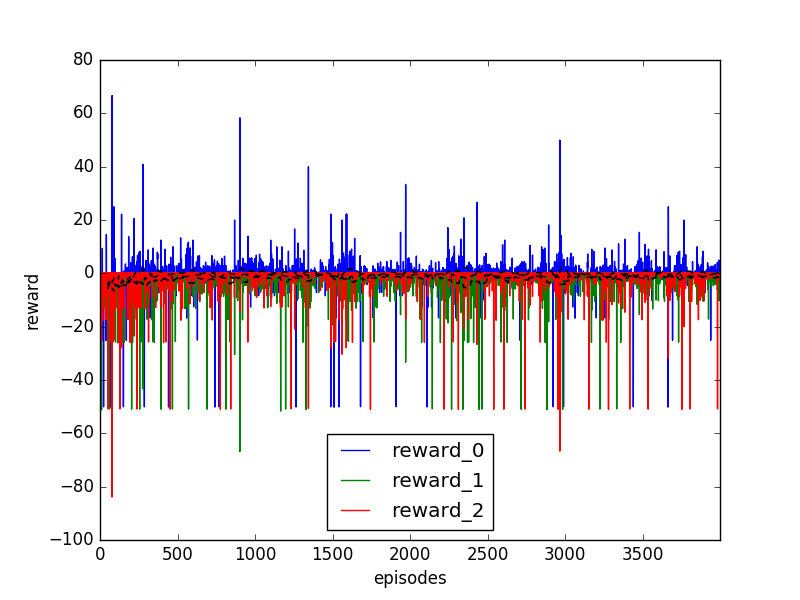
\includegraphics[trim=10 10 10 10,clip,width=\linewidth]
    {../results/dqn_2vs1/reward.png}
    \caption{Cumulative reward per episode over training episode for DQN.}
    \label{fig:dqn-2vs1-reward}
  \end{subfigure}
  ~
  \begin{subfigure}[h]{\figscale\linewidth}
    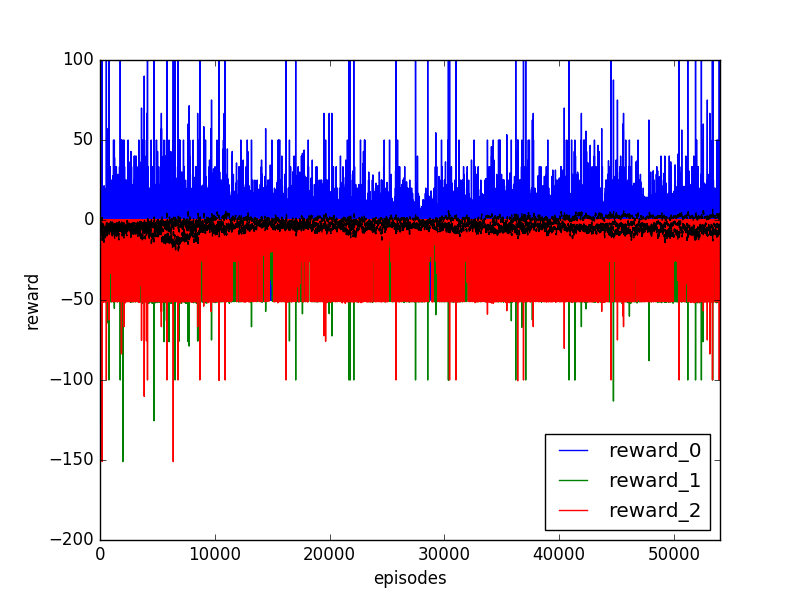
\includegraphics[trim=10 10 10 10,clip,width=\linewidth]
    {../results/ddpg_2vs1/reward.png}
    \caption{Cumulative reward per episode over training episode for DDPG.}
    \label{fig:ddpg-2vs1-reward}
  \end{subfigure}
  ~
  \begin{subfigure}[h]{\figscale\linewidth}
    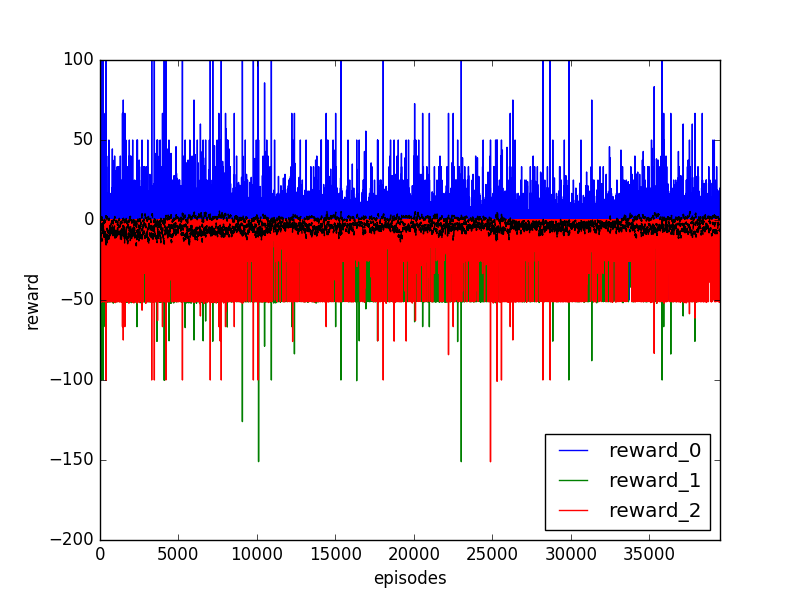
\includegraphics[trim=10 10 10 10,clip,width=\linewidth]
    {../results/maddpg_2vs1/reward.png}
    \caption{Cumulative reward per episode over training episode for MADDPG.}
    \label{fig:maddpg-2vs1-reward}
  \end{subfigure}

  \begin{subfigure}[h]{\figscale\linewidth}
    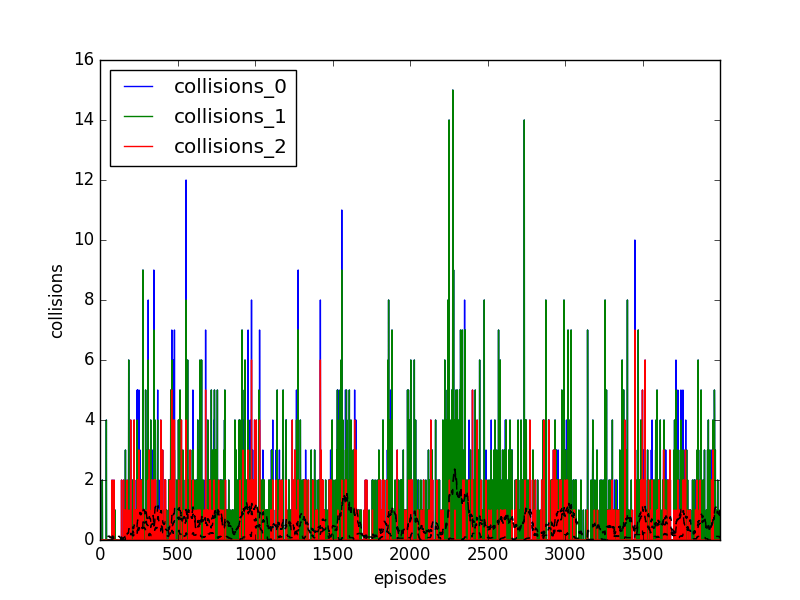
\includegraphics[trim=10 10 10 10,clip,width=\linewidth]
    {../results/dqn_2vs1/collisions.png}
    \caption{Number of collisions per episode over training episode for DQN.}
    \label{fig:dqn-2vs1-collisions}
  \end{subfigure}
  ~
  \begin{subfigure}[h]{\figscale\linewidth}
    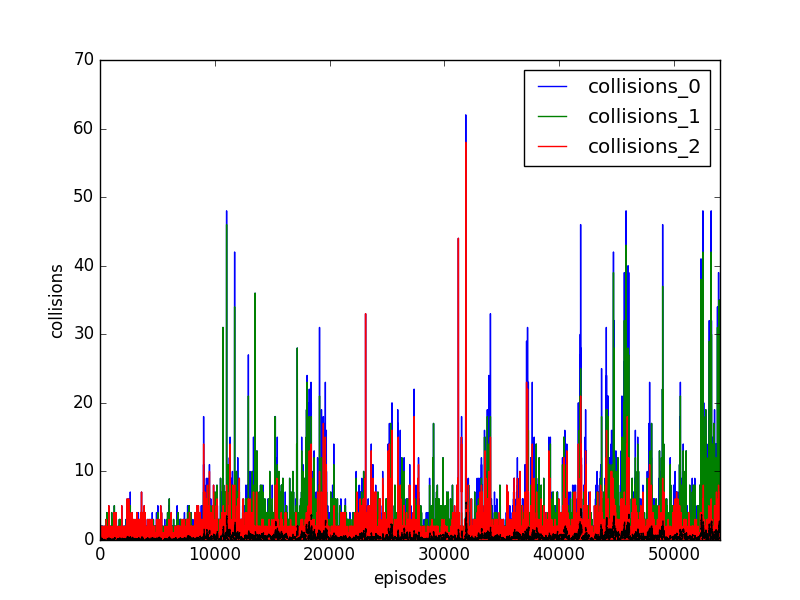
\includegraphics[trim=10 10 10 10,clip,width=\linewidth]
    {../results/ddpg_2vs1/collisions.png}
    \caption{Number of collisions per episode over training episode for DDPG.}
    \label{fig:ddpg-2vs1-collisions}
  \end{subfigure}
  ~
  \begin{subfigure}[h]{\figscale\linewidth}
    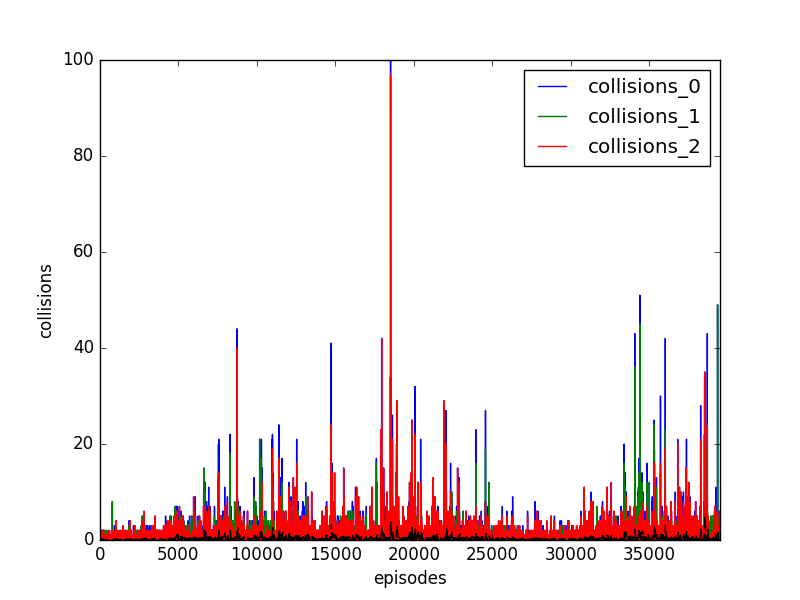
\includegraphics[trim=10 10 10 10,clip,width=\linewidth]
    {../results/maddpg_2vs1/collisions.png}
    \caption{Number of collisions per episode over training episode for MADDPG.}
    \label{fig:maddpg-2vs1-collisions}
  \end{subfigure}

  \begin{subfigure}[h]{\figscale\linewidth}
    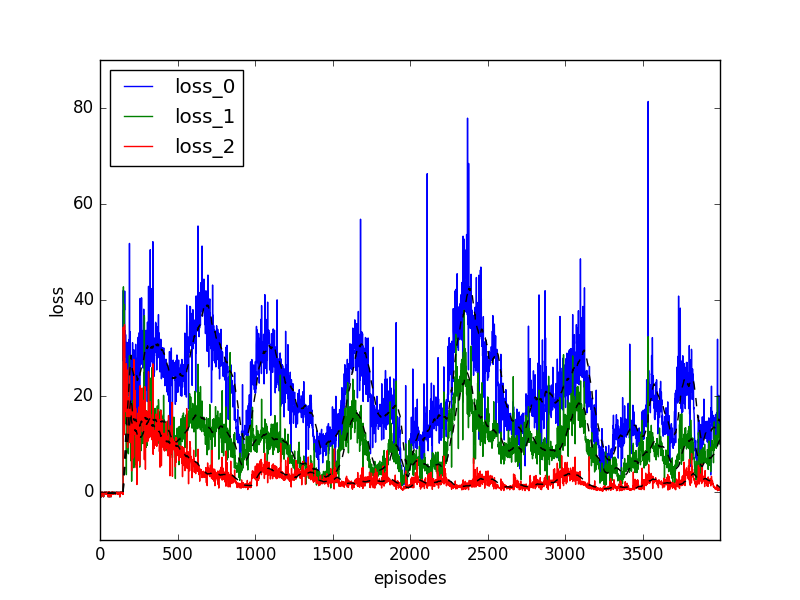
\includegraphics[trim=10 10 10 10,clip,width=\linewidth]
    {../results/dqn_2vs1/loss.png}
    \caption{Average loss per episode over training episode for DQN.}
    \label{fig:dqn-2vs1-loss}
  \end{subfigure}
  ~
  \begin{subfigure}[h]{\figscale\linewidth}
    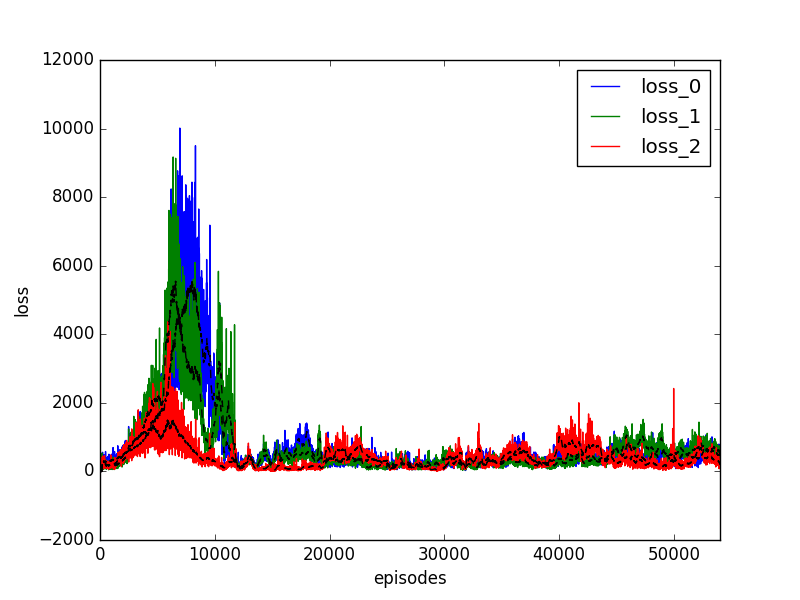
\includegraphics[trim=10 10 10 10,clip,width=\linewidth]
    {../results/ddpg_2vs1/loss.png}
    \caption{Average loss per episode over training episode for DDPG.}
    \label{fig:ddpg-2vs1-loss}
  \end{subfigure}
  ~
  \begin{subfigure}[h]{\figscale\linewidth}
    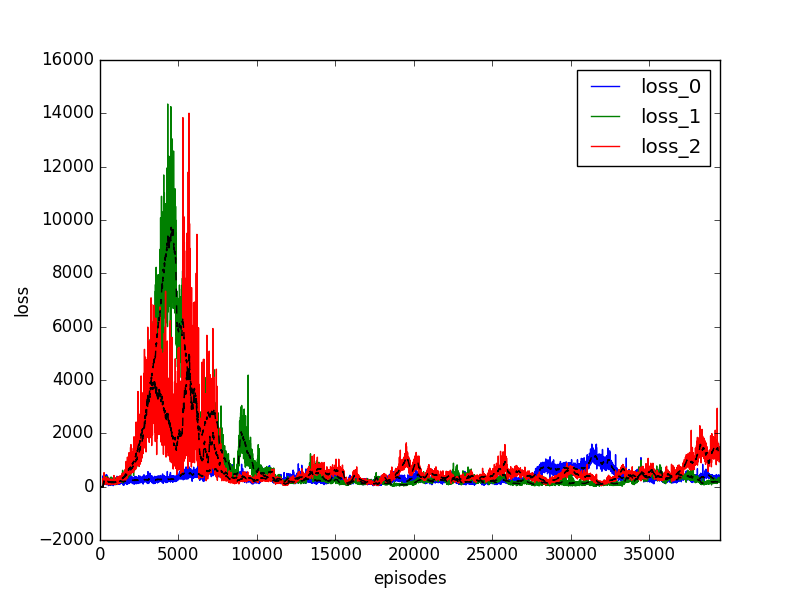
\includegraphics[trim=10 10 10 10,clip,width=\linewidth]
    {../results/maddpg_2vs1/loss.png}
    \caption{Average loss per episode over training episode for MADDPG.}
    \label{fig:maddpg-2vs1-loss}
  \end{subfigure}


  \caption{Results for predator-pray with one agent vs. two adversaries}
  \label{fig:2vs1}
\end{figure}
\FloatBarrier

